\documentclass[12pt, a4paper]{article}

%include packages
\usepackage{a4}
\usepackage[dvips]{graphicx}
\usepackage[ansinew]{inputenc}
\usepackage{epsfig}
\usepackage{amsmath}
\usepackage{amssymb}

\pagestyle{plain}
\pagenumbering{arabic}

\title{Real Valued Test Functions}
\author{Heuristic and Evolutionary Algorithms Laboratory (HEAL)}
\date{\today}

\begin{document}
	\maketitle

	\section*{Ackley Function}
		\begin{equation*}
			f(x) = 20 + e - 20 \cdot e^{\frac{1}{5} \sqrt{\frac{1}{n} \sum_{i=1}^n x_i^2}} - e^{\frac{1}{n} \sum_{i=1}^n \cos(2 \pi x_i)}
		\end{equation*}

		\begin{tabbing}
			\hspace{5cm}\=\kill
			\textbf{Dimensions:}     \> $n$ \\
			\textbf{Domain:}         \> $-32.768 \leq x_i \leq 32.768$ \\
			\textbf{Global Optimum:} \> $f(x) = 0.0$ at $x = (0.0, 0.0, \dots, 0.0)$ \\
			\textbf{Operator:}       \> AckleyEvaluator \\
			\textbf{Chart:}          \> \\
		\end{tabbing}

		\begin{center}
			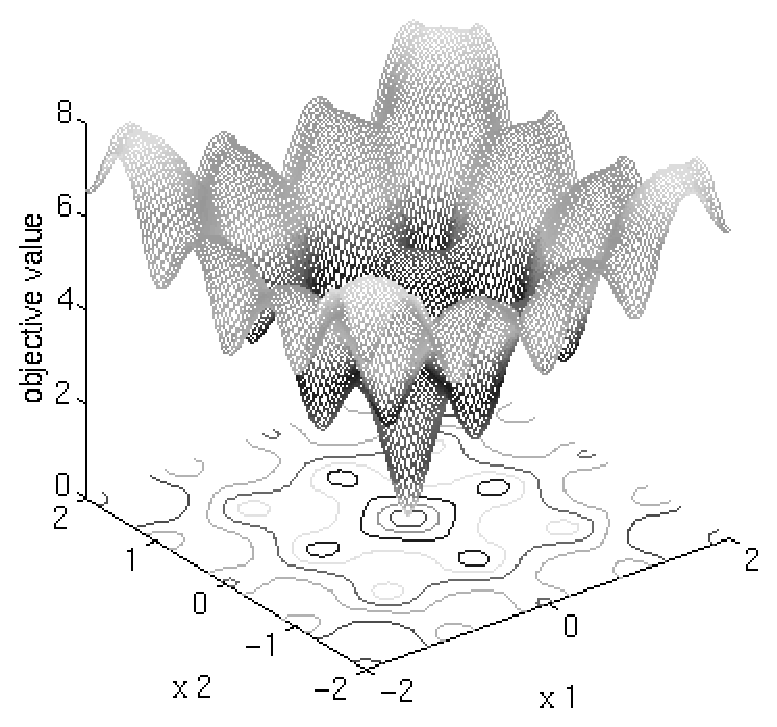
\includegraphics[width=0.6\textwidth]{Images/Ackley}
		\end{center}

	\section*{Beale Function}
		\begin{equation*}
			f(x) = (1.5 - x_1 (1 - x_2))^2 + (2.25 - x_1 (1 - x_2^2))^2 + (2.625 - x_1 (1 - x_2^3))^2
		\end{equation*}

		\begin{tabbing}
			\hspace{5cm}\=\kill
			\textbf{Dimensions:}     \> $2$ \\
			\textbf{Domain:}         \> $-4.5 \leq x_i \leq 4.5$ \\
			\textbf{Global Optimum:} \> $f(x) = 0.0$ at $x = (3.0, 0.5)$ \\
			\textbf{Operator:}       \> BealeEvaluator \\
			\textbf{Chart:}          \> \\
		\end{tabbing}

		\begin{center}
			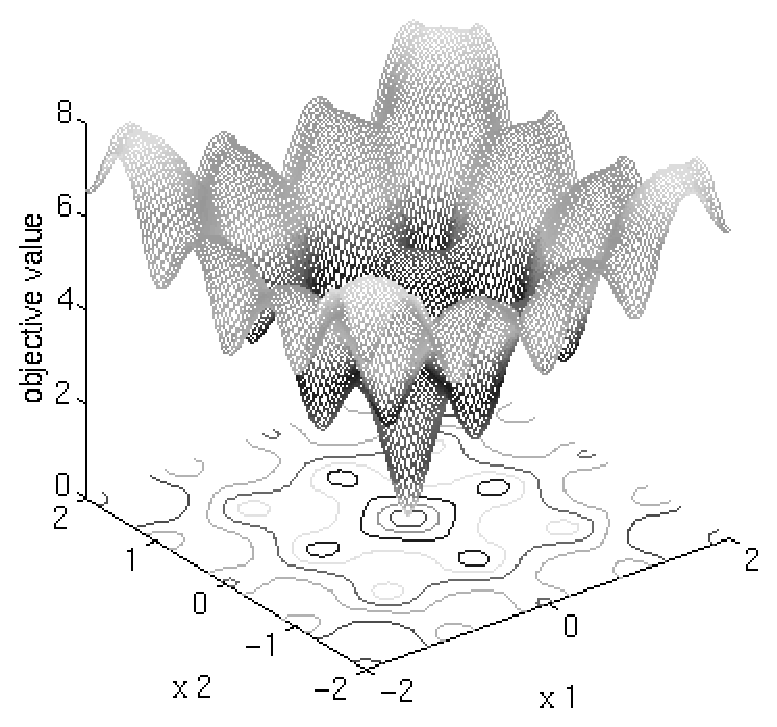
\includegraphics[width=0.6\textwidth]{Images/Ackley}
		\end{center}



\end{document}